\documentclass[12pt, a3j, dvipdfmx, jis2004]{jsarticle}
\usepackage[dvipdfmx]{graphicx}
\usepackage[margin=9truemm, bottom=18truemm]{geometry}
\usepackage[deluxe]{otf}
\special{}

\usepackage{amsmath, physics}
\usepackage{amssymb}
\usepackage{lipsum}


%色
\usepackage{xcolor}
\definecolor{lg}{rgb}{0.56, 0.93, 0.56} %lightgreen
\definecolor{color1}{rgb}{0.918, 0.402, 0.430}%赤
\definecolor{color2}{rgb}{0.883, 0.902, 0.387}%黄
\definecolor{color3}{rgb}{0.484, 0.750, 0.316}%緑
\definecolor{color4}{rgb}{0.378, 0.773, 0.879}%青
\definecolor{color5}{rgb}{0.664, 0.543, 0.746}%紫

\colorlet{thiscolor}{color4!150}	%テーマカラーの選択
\colorlet{linecolor}{thiscolor!150}
\colorlet{pagecolor}{thiscolor!40}
\pagecolor{pagecolor}


%ref
\usepackage[dvipdfmx, colorlinks = true, linkcolor = lg, urlcolor=blue, citecolor = lg, anchorcolor = lg]{hyperref}
\usepackage{pxjahyper, url}


%ヘッダーとフッター
\usepackage{fancyhdr}
\pagestyle{fancy}
\fancyhead{}
\fancyfoot[C]{\gtfamily\sffamily\textcolor{gray}{トポロジカル物性班\hfill\thepage}}
\renewcommand{\headrulewidth}{0pt}


%図
\usepackage{caption}
\usepackage{here}
\usepackage{wrapfig}
\captionsetup[figure]{format=plain, labelformat=simple, labelsep=period, font={sf, footnotesize}}
\renewcommand{\figurename}{Figure}
\renewcommand{\tablename}{Table}



%TikZ
\usepackage{tikz}
\usetikzlibrary{shapes.geometric}


%section関係
\usepackage{titlesec}
\titleformat{name=\section, numberless}
   [hang]
   {\vspace{2pt}\fontsize{20pt}{20pt}\selectfont}
   {\textcolor{linecolor}{■}}
   {3pt}
   {\hspace{0pt}}
   [\vspace{-5mm}\textcolor{linecolor}{\hrulefill}\vspace{-5mm}]


%tcolorbox
\usepackage{tcolorbox}
\tcbuselibrary{raster, skins}
\tcbset{	enhanced,
		colback=white,
		colframe=thiscolor!200,
		sharp corners,
		rounded corners = southeast,
		drop shadow,
		fonttitle=\gtfamily\sffamily\fontsize{15pt}{15pt}\selectfont,
		fontupper=\gtfamily\sffamily\fontsize{12pt}{12pt}\selectfont,
		before upper = \parindent 1zw,
		raster column skip = 5mm,
		raster row skip = 5mm,
		raster width center=\linewidth,
		raster valign=top}

%multicol
\usepackage{multicol}
\usepackage{comment}
\setlength{\columnsep}{5mm}
\newenvironment{twocols}{\begin{multicols}{2}[\vspace{-4mm}]}{\end{multicols}}
\newenvironment{twocols*}{\begin{multicols*}{2}[\vspace{-4mm}]}{\end{multicols*}}

%%%%%%%%%%%%%%%%%%%%%%%%%%%%%%%%%%%%%%%%%%%%%%%%
\begin{document}\sffamily\gtfamily

%%%%%%%%%%%%%%%%%%%%%%%%%%%%%%%%%%
\newpage
\section*{相転移現象としての超伝導}
\begin{tcbraster}[raster columns = 2, raster equal height = rows]
	\begin{tcolorbox}[title =相転移現象, raster multicolumn = 2]
		\begin{wrapfigure}{r}[0pt]{0.4\linewidth}
			\centering
			\vspace{-1zh}
			\includegraphics[height=0.5\linewidth]{picture/theo1.png}
			% \caption{水$\rightarrow$ 氷の相転移の様子}
			\end{wrapfigure}
		水が氷に変化するときのように系の性質が劇的に変化する現象を\textbf{相転移現象}といいます.水の場合は高温では水分子が動き回れるほうが安定であるため液体ですが,冷やすとじっとしていたほうが安定になるため氷になります.実は金属が超伝導になる現象も相転移として理解することができます.
	\end{tcolorbox}
%%%
	\begin{tcolorbox}[title=電子-格子相互作用]
		正電荷が格子点状に並んでいる空間を電子が通り過ぎる過程を考えましょう.
		\begin{figure}[H]
			\centering
			\vspace{-1zh}
			\includegraphics[height=0.4\linewidth]{picture/theo2.png}
			% \caption{電子が通ると正電荷が引き寄せられる}
		\end{figure}
		\vspace{-1zh}電子が通り過ぎると正電荷が電子に引き寄せられます.
		\begin{figure}[H]
			\centering
			\vspace{-1zh}
			\includegraphics[height=0.4\linewidth]{picture/theo3.png}
			% \caption{引き寄せられたところに正電荷がたまる}
		\end{figure}
		\vspace{-1zh}引き寄せられたところには+の電荷がたまっていて,後から来た電子はここに引き寄せられます.あたかも前の電子に後から来た電子が引き寄せられたように見ることができます.
	\end{tcolorbox}
%%%
	\begin{tcolorbox}[title = 超伝導のメカニズム]
	1911年に超伝導が水銀で発見されてから長い間超伝導のメカニズムは謎に包まれていました.しかし,本来はクーロン力によって反発しあうだけの電子の間にも左で説明したように仮想的な引力が働きうることがアメリカの物理学者クーパーによって示されました.ある種の金属の温度が転移温度以下になると,有効引力によって電子がペアを作り凝縮する相転移現象が起きます.このメカニズムを記述したのが1957年に発表された\textbf{BCS理論}です.BCS理論の完成を受けて超伝導のメカニズムに関する議論は一応の決着を見ました.
	\begin{figure}[H]
		\centering
		\vspace{-1zh}
		\includegraphics[height=0.3\linewidth]{picture/theo4.png}
		\caption{仮想的な引力で結ばれる電子対を\textbf{クーパー対}と呼びます}
	\end{figure}
	\end{tcolorbox}
%%%
	\begin{tcolorbox}[title = 巨視的波動関数(\texttt{High Level}), raster multicolumn = 2]
		\begin{wrapfigure}{l}[0pt]{0.5\linewidth}
			\centering
			\vspace{-2zh}
			\includegraphics[width=\linewidth]{picture/theo5.png}
			\caption{自発的に対称性が破れている状態といい,面白い物理がある}
			\end{wrapfigure}
			量子力学には位相の自由度があります.通常は各電子は位相を自由に取れて図の左側のようにバラバラの方向を向いています.しかし,超伝導転移が起きると全ての電子の位相が一方向に揃ってしまいます.この状態は巨視的な波動関数$\Psi$によって記述できます.
	\end{tcolorbox}
\end{tcbraster}



%%%%%%%%%%%%%%%%%%%%%%%%%%%%%%%%%%
\newpage
\section*{超伝導の実験事実}
\begin{tcbraster}[raster columns = 1]
	\begin{tcolorbox}[title = マイスナー効果]
		\begin{wrapfigure}{r}[0pt]{0.35\linewidth}
			\centering
			\vspace{-2zh}
			\includegraphics[height=1.2\linewidth]{picture/exp1.png}
			\caption{磁場中冷却による振る舞いの違い}
			\end{wrapfigure}
		超伝導は電気抵抗が$0$の現象として有名です.しかしこれは超伝導の本質なのでしょうか?電気抵抗が$0$の状態は他にも通常の金属の抵抗を連続的に$0$にもっていったものが考えられます.このような物質を完全導体と呼びます.まず,磁場がかかってない環境で超伝導体と完全導体に磁場をかけると,どちらも磁場を排除します.ここでの振る舞いの違いはありません.しかし,通常の金属の状態の時に磁場がかかっていると,温度を下げて超伝導/完全導体としたときに,超伝導体は磁場を排除しますが,完全導体を貫いた磁場はそのままとなります.\\
		超伝導体の性質を特徴づけているのは磁場に対する応答になります.このように能動的に超伝導体が磁場を排除するはたらきを\textbf{マイスナー効果}と呼びます.超伝導が通常の金属とは完全に異なる相にいるということを示しています.
	\end{tcolorbox}

%%%
	\begin{tcolorbox}[title = ジョセフソン効果]
		通常金属に電流を流すためには金属に電圧をかける必要があります.しかし,下の図のように二つの超伝導体をほんの少しだけ離しておくと電圧がかかっていないときにも電流が流れます.1962年にこの現象を予言したB.D. Josephsonの名前をとって\textbf{ジョセフソン効果}と呼ばれます.「相転移現象としての超伝導」で説明したように超伝導体の中ではすべての電子の位相が一方向にそろっています.二つの超伝導体を少しだけ離して置くと,一つの超伝導体になろうとして,二つの超伝導体の巨視的な位相の差に駆動されて電流が流れます.
		\begin{figure}[H]
			\centering
			% \vspace{-1zh}
			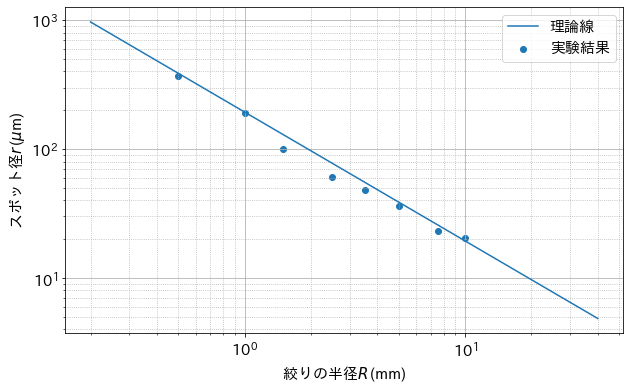
\includegraphics[height=0.3\linewidth]{picture/exp2.png}
			% \caption{電子が通ると正電荷が引き寄せられる}
		\end{figure}
	\end{tcolorbox}

	\begin{tcolorbox}[title = 超伝導に関する参考文献]
		\begin{thebibliography}{99}
			\bibitem  青木秀夫, 超伝導入門, 裳華房.
		\end{thebibliography}
		\end{tcolorbox}
\end{tcbraster}


\end{document}